%% abtex2-modelo-artigo.tex, v-1.9.5 laurocesar
%% Copyright 2012-2015 by abnTeX2 group at http://www.abntex.net.br/ 
%%
%% This work may be distributed and/or modified under the
%% conditions of the LaTeX Project Public License, either version 1.3
%% of this license or (at your option) any later version.
%% The latest version of this license is in
%%   http://www.latex-project.org/lppl.txt
%% and version 1.3 or later is part of all distributions of LaTeX
%% version 2005/12/01 or later.
%%
%% This work has the LPPL maintenance status `maintained'.
%% 
%% The Current Maintainer of this work is the abnTeX2 team, led
%% by Lauro César Araujo. Further information are available on 
%% http://www.abntex.net.br/
%%
%% This work consists of the files abntex2-modelo-artigo.tex and
%% abntex2-modelo-references.bib
%%

% ------------------------------------------------------------------------
% ------------------------------------------------------------------------
% abnTeX2: Modelo de Artigo Acadêmico em conformidade com
% ABNT NBR 6022:2003: Informação e documentação - Artigo em publicação 
% periódica científica impressa - Apresentação
% ------------------------------------------------------------------------
% ------------------------------------------------------------------------

\documentclass[
	% -- opções da classe memoir --
	article,			% indica que é um artigo acadêmico
	12pt,				% tamanho da fonte
	oneside,			% para impressão apenas no verso. Oposto a twoside
	a4paper,			% tamanho do papel. 
	% -- opções da classe abntex2 --
	%chapter=TITLE,		% títulos de capítulos convertidos em letras maiúsculas
	%section=TITLE,		% títulos de seções convertidos em letras maiúsculas
	%subsection=TITLE,	% títulos de subseções convertidos em letras maiúsculas
	%subsubsection=TITLE % títulos de subsubseções convertidos em letras maiúsculas
	% -- opções do pacote babel --
	english,			% idioma adicional para hifenização
	brazil,				% o último idioma é o principal do documento
	sumario=tradicional
	]{abntex2}


% ---
% PACOTES
% ---

% ---
% Pacotes fundamentais 
% ---
\usepackage{lmodern}			% Usa a fonte Latin Modern
\usepackage[T1]{fontenc}		% Selecao de codigos de fonte.
\usepackage[utf8]{inputenc}		% Codificacao do documento (conversão automática dos acentos)
\usepackage{indentfirst}		% Indenta o primeiro parágrafo de cada seção.
\usepackage{nomencl} 			% Lista de simbolos
\usepackage{color}				% Controle das cores
\usepackage{graphicx}			% Inclusão de gráficos
\usepackage{microtype} 			% para melhorias de justificação
% ---
		
% ---
% Pacotes adicionais, usados apenas no âmbito do Modelo Canônico do abnteX2
% ---
% \usepackage{lipsum}
% ---
% Pacotes de citações
% ---
% ---



% ---
% Informações de dados para CAPA e FOLHA DE ROSTO
% ---
% \titulo{Projeto Final de Programação Orientada a Objetos 2}
% \autor{Autor: Caio Pereira Oliveira
% \\Equipe: João Victor Fagundes e Caio Pereira Oliveira}
% \local{UFSC}
% \data{1/12/2015}
% ---

% ---
% Configurações de aparência do PDF final

% alterando o aspecto da cor azul

% informações do PDF
\makeatletter
\hypersetup{
     	%pagebackref=true,
		pdftitle={\@title}, 
		pdfauthor={\@author},
    	pdfsubject={Pokemon Team Builder},
	    pdfcreator={LaTeX with abnTeX2},
		pdfkeywords={abnt}{latex}{abntex}{abntex2}{atigo científico}, 
		colorlinks=true,       		% false: boxed links; true: colored links
    	linkcolor=blue,          	% color of internal links
    	citecolor=blue,        		% color of links to bibliography
    	filecolor=magenta,      		% color of file links
		urlcolor=blue,
		bookmarksdepth=4
}
\makeatother
% --- 

% ---
% compila o indice
% ---
\makeindex
% ---

% ---
% Altera as margens padrões
% ---
\setlrmarginsandblock{3cm}{3cm}{*}
\setulmarginsandblock{3cm}{3cm}{*}
\checkandfixthelayout
% ---

% --- 
% Espaçamentos entre linhas e parágrafos 
% --- 

% O tamanho do parágrafo é dado por:
\setlength{\parindent}{1.3cm}

% Controle do espaçamento entre um parágrafo e outro:
\setlength{\parskip}{0.2cm}  % tente também \onelineskip

% Espaçamento simples
\SingleSpacing

% ----
% Início do documento
% ----
\begin{document}

% Seleciona o idioma do documento (conforme pacotes do babel)
%\selectlanguage{english}
\selectlanguage{brazil}

% Retira espaço extra obsoleto entre as frases.
\frenchspacing 

% ----------------------------------------------------------
% ELEMENTOS PRÉ-TEXTUAIS
% ----------------------------------------------------------

%---
%
% Se desejar escrever o artigo em duas colunas, descomente a linha abaixo
% e a linha com o texto ``FIM DE ARTIGO EM DUAS COLUNAS''.
% \twocolumn[    		% INICIO DE ARTIGO EM DUAS COLUNAS
%
%---
% página de titulo

% \centering

\begin{center}

\includegraphics[width=0.30\textwidth]{brasao_ufsc}\par\vspace{1cm}
{\scshape\LARGE Universidade Federal de Santa Catarina \par}
\vspace{1cm}
{\scshape\Large Projeto Final de Programação Orientada a Objetos\par}
\vspace{1.5cm}
{\huge\bfseries Pokémon Team Builder\par}
\vspace{2cm}
{\Large\itshape Autor: Caio Pereira Oliveira\\Equipe: Caio Pereira Oliveira e João Victor Fagundes\par}
\vfill
{\Large Professor: Rosvelter J. C. da Costa}

% \vfill
\vspace{\fill}
{\large \today\par}

\end{center}

\textual

% ----------------------------------------------------------
% Introdução
% ----------------------------------------------------------
\newpage
\section*{}

\begin{center}
{\HUGE Introdução}
\end{center}
% \addcontentsline{toc}{section}{Introdução}

Pokémon é uma franquia de jogos muito popular, seu primeiro lançado em 1995, fazendo bastante sucesso desde então. O objetivo dos jogos de Pokémon é capturar e treinar monstros (Pokémons), formando equipes de até 6 Pokémons, para batalhar com outros treinadores. Com este sucesso da franquia, muitas pessoas se dedicam a criar times de Pokémons cada vez melhores para enfrentar e ganhar de outros treinadores. Pensando nisso, nossa equipe elaborou um montador de equipes de Pokémon, para que treinadores possam planejar suas equipes vencedoras.


\begin{center}
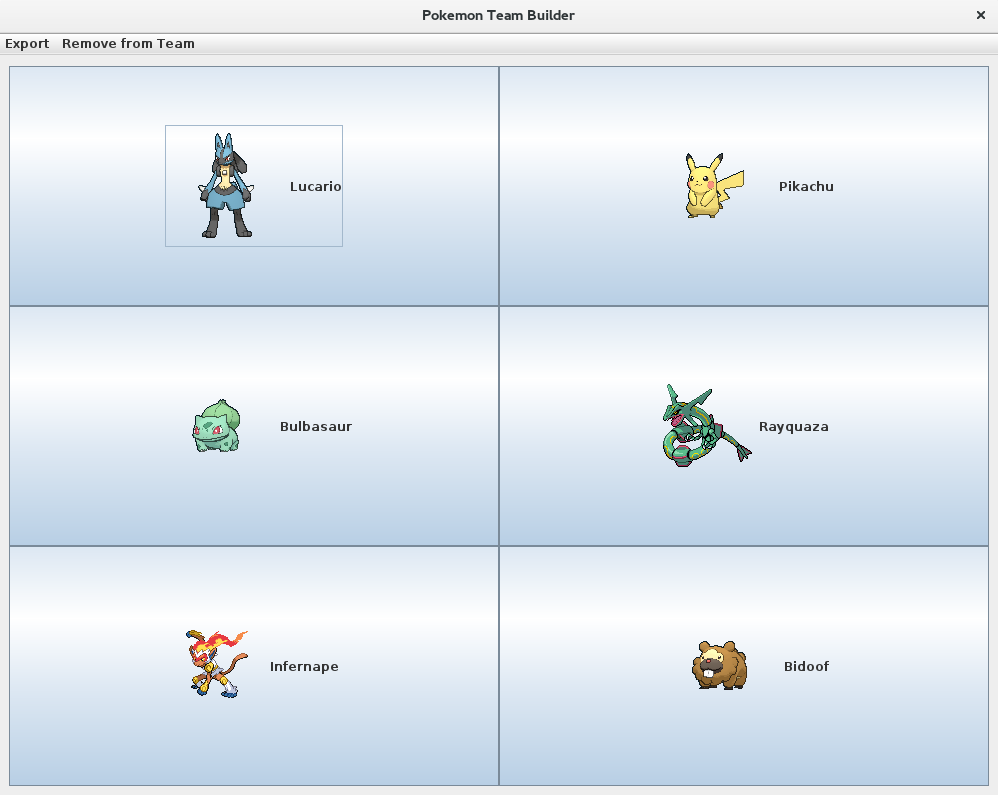
\includegraphics[width=1\textwidth]{team_full}\par\vspace{1cm}
\end{center}




\newpage
\section*{}

\begin{center}
{\HUGE Uso do programa}
\end{center}

A navegação através pelo programa é feita através de menus.

\begin{center}
{\Large Menu Principal}
\end{center}

No menu principal, existem 3 opções para o usuário:

\begin{center}
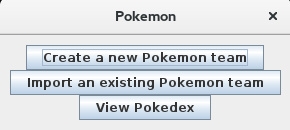
\includegraphics[width=0.5\textwidth]{menu}\par\vspace{1cm}
\end{center}

\begin{itemize}

{\item\bfseries Create a new Pokemon team}: Cria um novo time de Pokémon vazio.

{\item\bfseries Import an existing Pokémon team}: Importa um time de Pokémon previamente exportado.

{\item\bfseries View Pokedéx}: Abre a Pokedéx (lista de todos os Pokémons existentes).

\end{itemize}

Ao escolher {\bfseries Create a new Pokemon team}, o programa abrirá a janela de montagem de time com um novo time vazio.

Escolhendo {\bfseries Import an existing Pokémon team} o usuário deverá escolher um arquivo de time previamente exportando, e então o programa abrirá a janela de montagem de time com o time importado.

E ao escolher {\bfseries View Pokedéx}, será aberta a janela da Pokédex, que contém uma lista de todos os Pokémons.

\newpage
\begin{center}
{\Large Montador de time}
\end{center}



\begin{center}
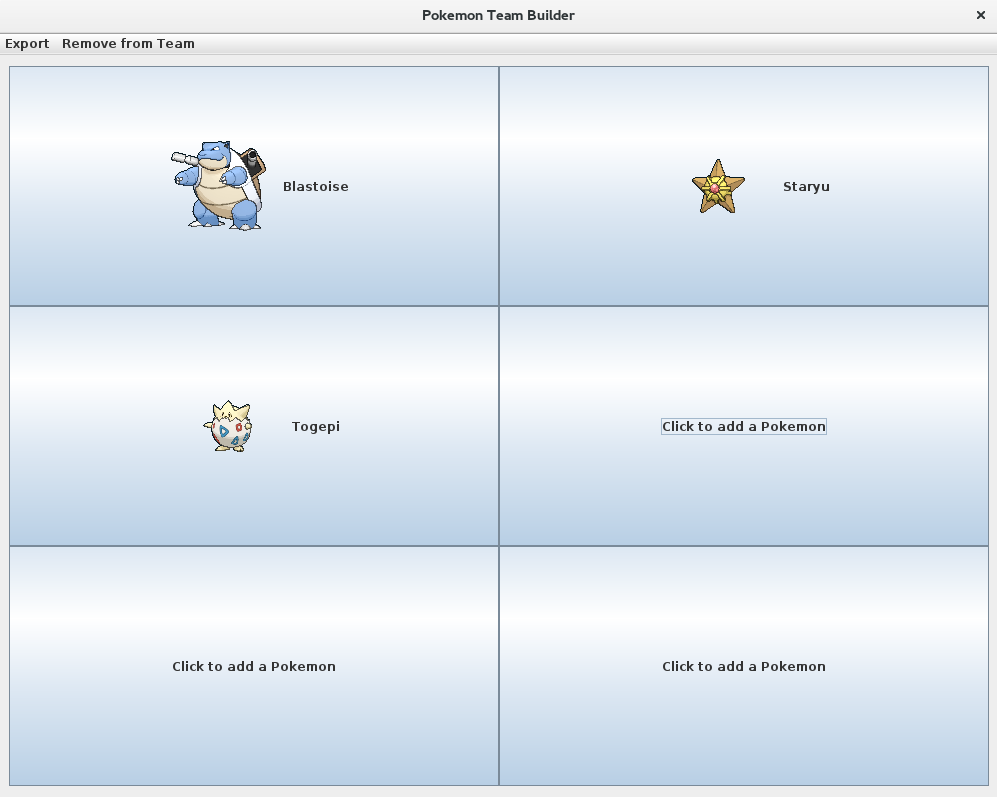
\includegraphics[width=1\textwidth]{team_half}\par\vspace{1cm}
\end{center}



% \begin{center}
% 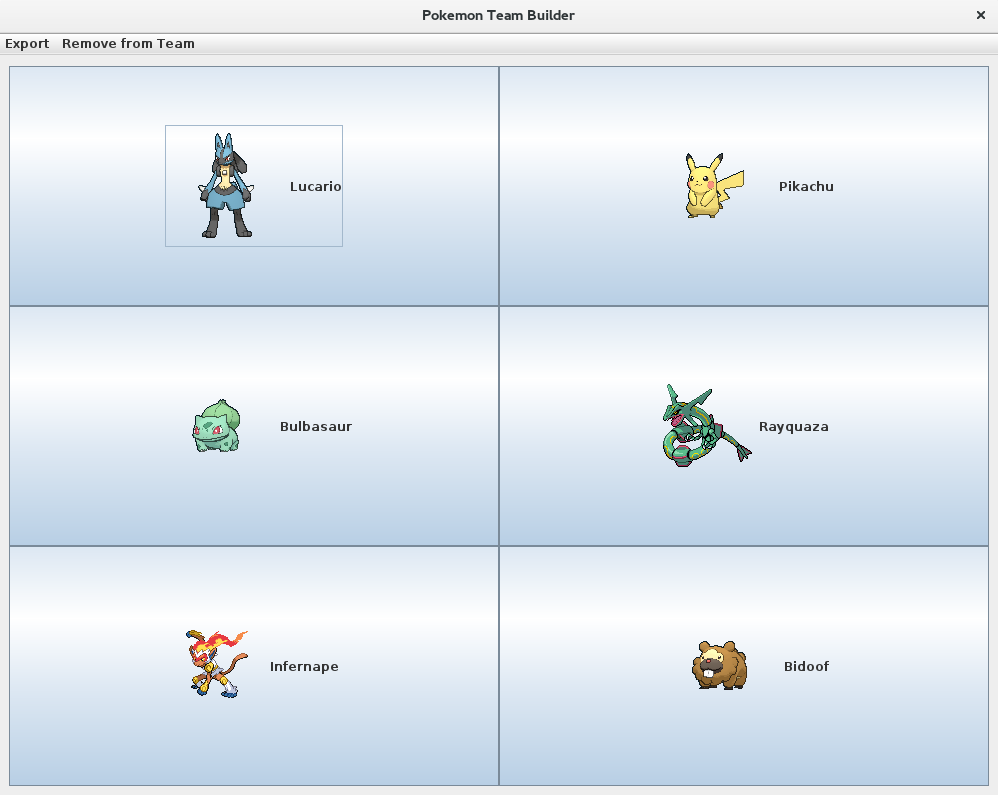
\includegraphics[width=1\textwidth]{team_full}\par\vspace{1cm}
% \end{center}



\end{document}
